%% Beginning of file 'sample7.tex'
%%
%% Version 7. Created January 2025.  
%%
%% AASTeX v7 calls the following external packages:
%% times, hyperref, ifthen, hyphens, longtable, xcolor, 
%% bookmarks, array, rotating, ulem, and lineno 
%%
%% RevTeX is no longer used in AASTeX v7.
%%
\documentclass[linenumbers,trackchanges]{aastex7}
%%
%% This initial command takes arguments that can be used to easily modify 
%% the output of the compiled manuscript. Any combination of arguments can be 
%% invoked like this:
%%
%% \documentclass[argument1,argument2,argument3,...]{aastex7}
%%
%% Six of the arguments are typestting options. They are:
%%
%%  twocolumn   : two text columns, 10 point font, single spaced article.
%%                This is the most compact and represent the final published
%%                derived PDF copy of the accepted manuscript from the publisher
%%  default     : one text column, 10 point font, single spaced (default).
%%  manuscript  : one text column, 12 point font, double spaced article.
%%  preprint    : one text column, 12 point font, single spaced article.  
%%  preprint2   : two text columns, 12 point font, single spaced article.
%%  modern      : a stylish, single text column, 12 point font, article with
%% 		  wider left and right margins. This uses the Daniel
%% 		  Foreman-Mackey and David Hogg design.
%%
%% Note that you can submit to the AAS Journals in any of these 6 styles.
%%
%% There are other optional arguments one can invoke to allow other stylistic
%% actions. The available options are:
%%
%%   astrosymb    : Loads Astrosymb font and define \astrocommands. 
%%   tighten      : Makes baselineskip slightly smaller, only works with 
%%                  the twocolumn substyle.
%%   times        : uses times font instead of the default.
%%   linenumbers  : turn on linenumbering. Note this is mandatory for AAS
%%                  Journal submissions and revisions.
%%   trackchanges : Shows added text in bold.
%%   longauthor   : Do not use the more compressed footnote style (default) for 
%%                  the author/collaboration/affiliations. Instead print all
%%                  affiliation information after each name. Creates a much 
%%                  longer author list but may be desirable for short 
%%                  author papers.
%% twocolappendix : make 2 column appendix.
%%   anonymous    : Do not show the authors, affiliations, acknowledgments,
%%                  and author contributions for dual anonymous review.
%%  resetfootnote : Reset footnotes to 1 in the body of the manuscript.
%%                  Useful when there are a lot of authors and affiliations
%%		    in the front matter.
%%   longbib      : Print article titles in the references. This option
%% 		    is mandatory for PSJ manuscripts.
%%
%% Since v6, AASTeX has included \hyperref support. While we have built in 
%% specific %% defaults into the classfile you can manually override them 
%% with the \hypersetup command. For example,
%%
%% \hypersetup{linkcolor=red,citecolor=green,filecolor=cyan,urlcolor=magenta}
%%
%% will change the color of the internal links to red, the links to the
%% bibliography to green, the file links to cyan, and the external links to
%% magenta. Additional information on \hyperref options can be found here:
%% https://www.tug.org/applications/hyperref/manual.html#x1-40003
%%
%% The "bookmarks" has been changed to "true" in hyperref
%% to improve the accessibility of the compiled pdf file.
%%
%% If you want to create your own macros, you can do so
%% using \newcommand. Your macros should appear before
%% the \begin{document} command.
%%
\newcommand{\vdag}{(v)^\dagger}
\newcommand\aastex{AAS\TeX}
\newcommand\latex{La\TeX}
% RMH commands
%%%%%%%%%%%%%%%%%%%%%%%%%%
% FOR PUBLISHING UNCOMMENT THIS LINE
% \newcommand{\TEMP}[1]{}
%%%%%%%%%%%%%%%%%%%%%%%%%%
% FOR WRITING UNCOMMENT THIS LINE
\newcommand{\TEMP}[1]{#1}
%%%%%%%%%%%%%%%%%%%%%%%%%%
\newcommand{\COM}[1]{\TEMP{\textbf{\textcolor{red}{COMMENT}}: \textit{#1}}}
\newcommand{\REMOVED}[1]{\TEMP{\textit{\textcolor{gray}{#1}}}}
\newcommand{\ADDED}[1]{\TEMP{\textcolor{red}{#1}}}
% RMH variables
\newcommand{\DeltaBIC}[0]{$\Delta\mathrm{BIC}$}
%%%%%%%%%%%%%%%%%%%%%%%%%%%%%%%%%%%%%%%%%%%%%%%%%%%%%%%%%%%%%%%%%%%%%%%%%%%%%%%%
%%
%% The following section outlines numerous optional output that
%% can be displayed in the front matter or as running meta-data.
%%
%% Running header information. A short title on odd pages and 
%% short author list on even pages. Note that this
%% information may be modified in production.
%%\shorttitle{AASTeX v7 Sample article}
%%\shortauthors{The Terra Mater collaboration}
%%
%% Include dates for submitted, revised, and accepted.
%%\received{February 1, 2025}
%%\revised{March 1, 2025}
%%\accepted{\today}
%%
%% Indicate AAS Journal the manuscript was submitted to.
%%\submitjournal{PSJ}
%% Note that this command adds "Submitted to " the argument.
%%
%% You can add a light gray and diagonal water-mark to the first page 
%% with this command:
%% \watermark{text}
%% where "text", e.g. DRAFT, is the text to appear.  If the text is 
%% long you can control the water-mark size with:
%% \setwatermarkfontsize{dimension}
%% where dimension is any recognized LaTeX dimension, e.g. pt, in, etc.
%%%%%%%%%%%%%%%%%%%%%%%%%%%%%%%%%%%%%%%%%%%%%%%%%%%%%%%%%%%%%%%%%%%%%%%%%%%%%%%%
%%

%% packages added by RMH
\usepackage{float}

%% Use this command to indicate a subdirectory where figures are located.
%%\graphicspath{{./}{figures/}}
%% This is the end of the preamble.  Indicate the beginning of the
%% manuscript itself with \begin{document}.

\begin{document}

\title{Searching for Non-Keplerian Orbital Motion in the HAT-P-37 Hot Jupiter System with the Help of Transit Observations by Small Telescopes}

%% Due to the length of the author list, it is corralled into it's own tex file. 
%% A significant change from AASTeX v6+ is in the author blocks. Now an email
%% address is required for each author. This means that each author requires
%% at least one of the following:
%%
%% \author
%% \affiliation
%% \email
%%
%% Even though emails are now required for each author, the \email does not
%% produce output in the compiled manuscript unless the optional "show" command
%% is used. For example,
%%
%% \email[show]{greg.schwarz@aas.org}
%%
%% All "shown" emails are show in the bottom left of the first page. Due to
%% space constraints, only a few emails should be shown. 
%%
%% To identify a corresponding author, use the \correspondingauthor command.
%% The command appends "Corresponding Author: " to the argument it appears at
%% the bottom left of the first page like the output from \email. 
\author[0000-0002-3548-1655]{Rachel M.~Huchmala}
\affiliation{Schmid College of Science and Technology, Chapman University, Orange, CA, USA.}
\affiliation{Department of Physics, Boise State University, 1910 University Drive, Boise ID 83725-1570 USA}
\email[show]{huchmala@chapman.edu}

\author[0000-0001-6629-5399]{Lauren A.~Sgro}
\affiliation{SETI Institute, Carl Sagan Center, 339 Bernardo Ave., Suite 200, Mountain View, CA 94043, USA}
\email{lsgro@seti.org}

\author[]{Heather B.~Hewitt}
\affiliation{School of Earth and Space Exploration, Arizona State University, 781 E. Terrace Mall, Tempe, AZ 85287-6004}
\email{hbhewitt@asu.edu}

\author[]{Federico R.~Noguer}
\affiliation{School of Earth and Space Exploration, Arizona State University, 781 E. Terrace Mall, Tempe, AZ 85287-6004}
\email{fnoguer@asu.edu}

\author[0000-0002-9495-9700]{Brian Jackson}
\affiliation{Department of Physics, Boise State University, 1910 University Drive, Boise ID 83725-1570 USA}
\affiliation{SETI Institute, Carl Sagan Center, 339 Bernardo Ave., Suite 200, Mountain View, CA 94043, USA}
\email{bjackson@boisestate.edu}

\author[0000-0002-9131-5969]{Elisabeth R.~Adams}
\affiliation{Planetary Science Institute, 1700 E. Ft. Lowell, Suite 106, Tucson, AZ 85719, USA}
\email{adams@psi.edu}

\author[0000-0002-9495-9700]{Malia Barker}
\affiliation{Department of Physics, Boise State University, 1910 University Drive, Boise ID 83725-1570 USA}
\affiliation{Department of Computer Science, Boise State University, 1910 University Drive, Boise ID 83725-1570 USA}
\email{maliabarker@u.boisestate.edu}

\author[0000-0003-3716-3455]{Jeffrey P.~Morgenthaler}
\email{morgenthaler@psi.edu}
\affiliation{Planetary Science Institute, 1700 E. Ft. Lowell, Suite 106, Tucson, AZ 85719, USA}

\author[0000-0002-9468-7477]{Amanda A.~Sickafoose}
\email{sickafoose@psi.edu}
\affiliation{Planetary Science Institute, 1700 E. Ft. Lowell, Suite 106, Tucson, AZ 85719, USA}

%% The following authors are being cited for their observational contributions to this paper, and will not neccessarily be involved in the writing/editing of this paper.

\author[]{Greg Harmon}
\email{}
\affiliation{Bruneau Dunes State Park}

\author[]{Dallon Carlson}
\email{}
\affiliation{Department of Physics, Boise State University, 1910 University Drive, Boise ID 83725-1570 USA}

\author[]{Hailey Stubbers}
\email{}
\affiliation{Department of Physics, Boise State University, 1910 University Drive, Boise ID 83725-1570 USA}

\author[]{Killian Richardson}
\email{}
\affiliation{Department of Physics, Boise State University, 1910 University Drive, Boise ID 83725-1570 USA}

\author[]{Bradley Fick}
\email{}
\affiliation{Department of Physics, Boise State University, 1910 University Drive, Boise ID 83725-1570 USA}

\author[]{Sean Buck}
\email{}
\affiliation{Department of Physics, Boise State University, 1910 University Drive, Boise ID 83725-1570 USA}

\author[]{Janna Artiles Ramos}
\email{}
\affiliation{Department of Physics, Boise State University, 1910 University Drive, Boise ID 83725-1570 USA}

\author[]{Nathaniel Baumann}
\email{}
\affiliation{Department of Physics, Boise State University, 1910 University Drive, Boise ID 83725-1570 USA}

\author[]{Anna Humphrey}
\email{}
\affiliation{Department of Physics, Boise State University, 1910 University Drive, Boise ID 83725-1570 USA}

\author[]{Nathan Silvey}
\email{}
\affiliation{Department of Physics, Boise State University, 1910 University Drive, Boise ID 83725-1570 USA}

\author[]{Rachel Clark}
\email{}
\affiliation{Department of Physics, Boise State University, 1910 University Drive, Boise ID 83725-1570 USA}




%% Mark off the abstract in the ``abstract'' environment. 
\begin{abstract}

HAT-P-37 b is a Hot Jupiter with an approximate 2.8 day period around a 0.9 solar mass G-type star. Recent studies of HAT-P-37 b have shown it exhibits transit timing variations (TTVs) most recently compared to a precession model. In this work, we present a total of X new midtimes for HAT-P-37 b. These results are a combination of transit observations from TESS, the on-campus observatory at Boise State University, \COM{ASU transits,} and from amateur astronomers \COM{only Unistellar?} to increase the observational baseline of HAT-P-37 b in an effort to distinguish the cause of the transit timing variation. \COM{Potentially add the \DeltaBIC ??}

\end{abstract}

%% Keywords should appear after the \end{abstract} command. 
%% The AAS Journals now uses Unified Astronomy Thesaurus (UAT) concepts:
%% https://astrothesaurus.org
%% You will be asked to selected these concepts during the submission process
%% but this old "keyword" functionality is maintained in case authors want
%% to include these concepts in their preprints.
%%
%% You can use the \uat command to link your UAT concepts back its source.
\keywords{\uat{Exoplanet dynamics}{490} --- \uat{Exoplanet tides}{497} --- \uat{Transit timing variation method}{1710} --- \uat{Star-planet interactions}{2177} --- \uat{Stellar astronomy}{1583} --- \uat{Solar physics}{1476}}

%% From the front matter, we move on to the body of the paper.
%% Sections are demarcated by \section and \subsection, respectively.
%% Observe the use of the LaTeX \label
%% command after the \subsection to give a symbolic KEY to the
%% subsection for cross-referencing in a \ref command.
%% You can use LaTeX's \ref and \label commands to keep track of
%% cross-references to sections, equations, tables, and figures.
%% That way, if you change the order of any elements, LaTeX will
%% automatically renumber them.

\section{Introduction} \label{sec:Intro}
\input{introduction}

\section{Data} \label{sec:data}

\subsection{TESS database} \label{sec:tessData}
\COM{58 midtimes - new analysis, 19 midtimes - Elisabeth (S74/75), 8 midtimes - Wang (S59)}
The HAT-P-37 system is present in 11 different sectors of TESS with a cadence of 120.0 s. Previously timing data from only one sector (59) has been published. \cite{wangLongtermVariationsOrbital2024} Upon investigation, 9 out of the 10 unpublished sector lightcurves produced by the TESS-SPOC pipeline in the lightkurve package show significant contamination of the HAT-P-37 flux. Using the MAST database(?), we were able to determine that the main source of this contamination was a nearby variable star, ZTFJ185715.34+511631.4, which is a W Ursae Majoris (EW)-type Eclipsing binary, as characterized by Chen et. al.\citep{chenZwickyTransientFacility2020}. For simplicity, we will refer to this star as "EB" from here on. 

Using the orbital period from Chen et. al. and the tools in the lightkurve package, we have been able to separate the transit light curves for HAT-P-37 b from the variability of the EB. Figure \ref{fig:EB_folded} depicts all 11 sector's PDCSAP flux phase folded to the parameters of the EB as published previously. This figure shows that the amount of contamination varies from sector to sector, leading to a sector specific approach being necessary to remove the contamination and fit the transit light curves of HAT-P-37 b.

\begin{figure}
    \centering
    \includegraphics[width=0.9\linewidth]{figures/all_sectors_folded_EB_period.png}
    \caption{TESS sectors phase folded on the period of the EB. Each sector is affected by a different amount of contamination and as such each sector will need to be detrended separately.}
    \label{fig:EB_folded}
\end{figure}

TESS Sector used in this study: 

\begin{itemize}
    \item 26 - Average fraction of flux of the target star:  76.932538 \%
    \item 40 - Average fraction of flux of the target star:  65.78933599999999 \%
    \item 41 - Average fraction of flux of the target star:  66.98885 \%
    \item 53 - Average fraction of flux of the target star:  60.779458 \%
    \item 54 - Average fraction of flux of the target star:  64.582843 \%
    \item 55 - Average fraction of flux of the target star:  74.128646 \%
    \item 59 - large dip approx. 12 day period, masked in PDCSAP flux, but probably need to look into what it is - Average fraction of flux of the target star:  58.385509 \%
    \item 74 - no contamination with EB - fit fine as it - Average fraction of flux of the target star:  59.20288 \%
    \item 75 - no contamination with EB - fit fine as it - Average fraction of flux of the target star:  59.999548999999995 \%
    \item 80 - Average fraction of flux of the target star:  65.208763 \%
    \item 82 - Average fraction of flux of the target star:  66.821003 \%
\end{itemize}

\begin{figure}
    \centering
    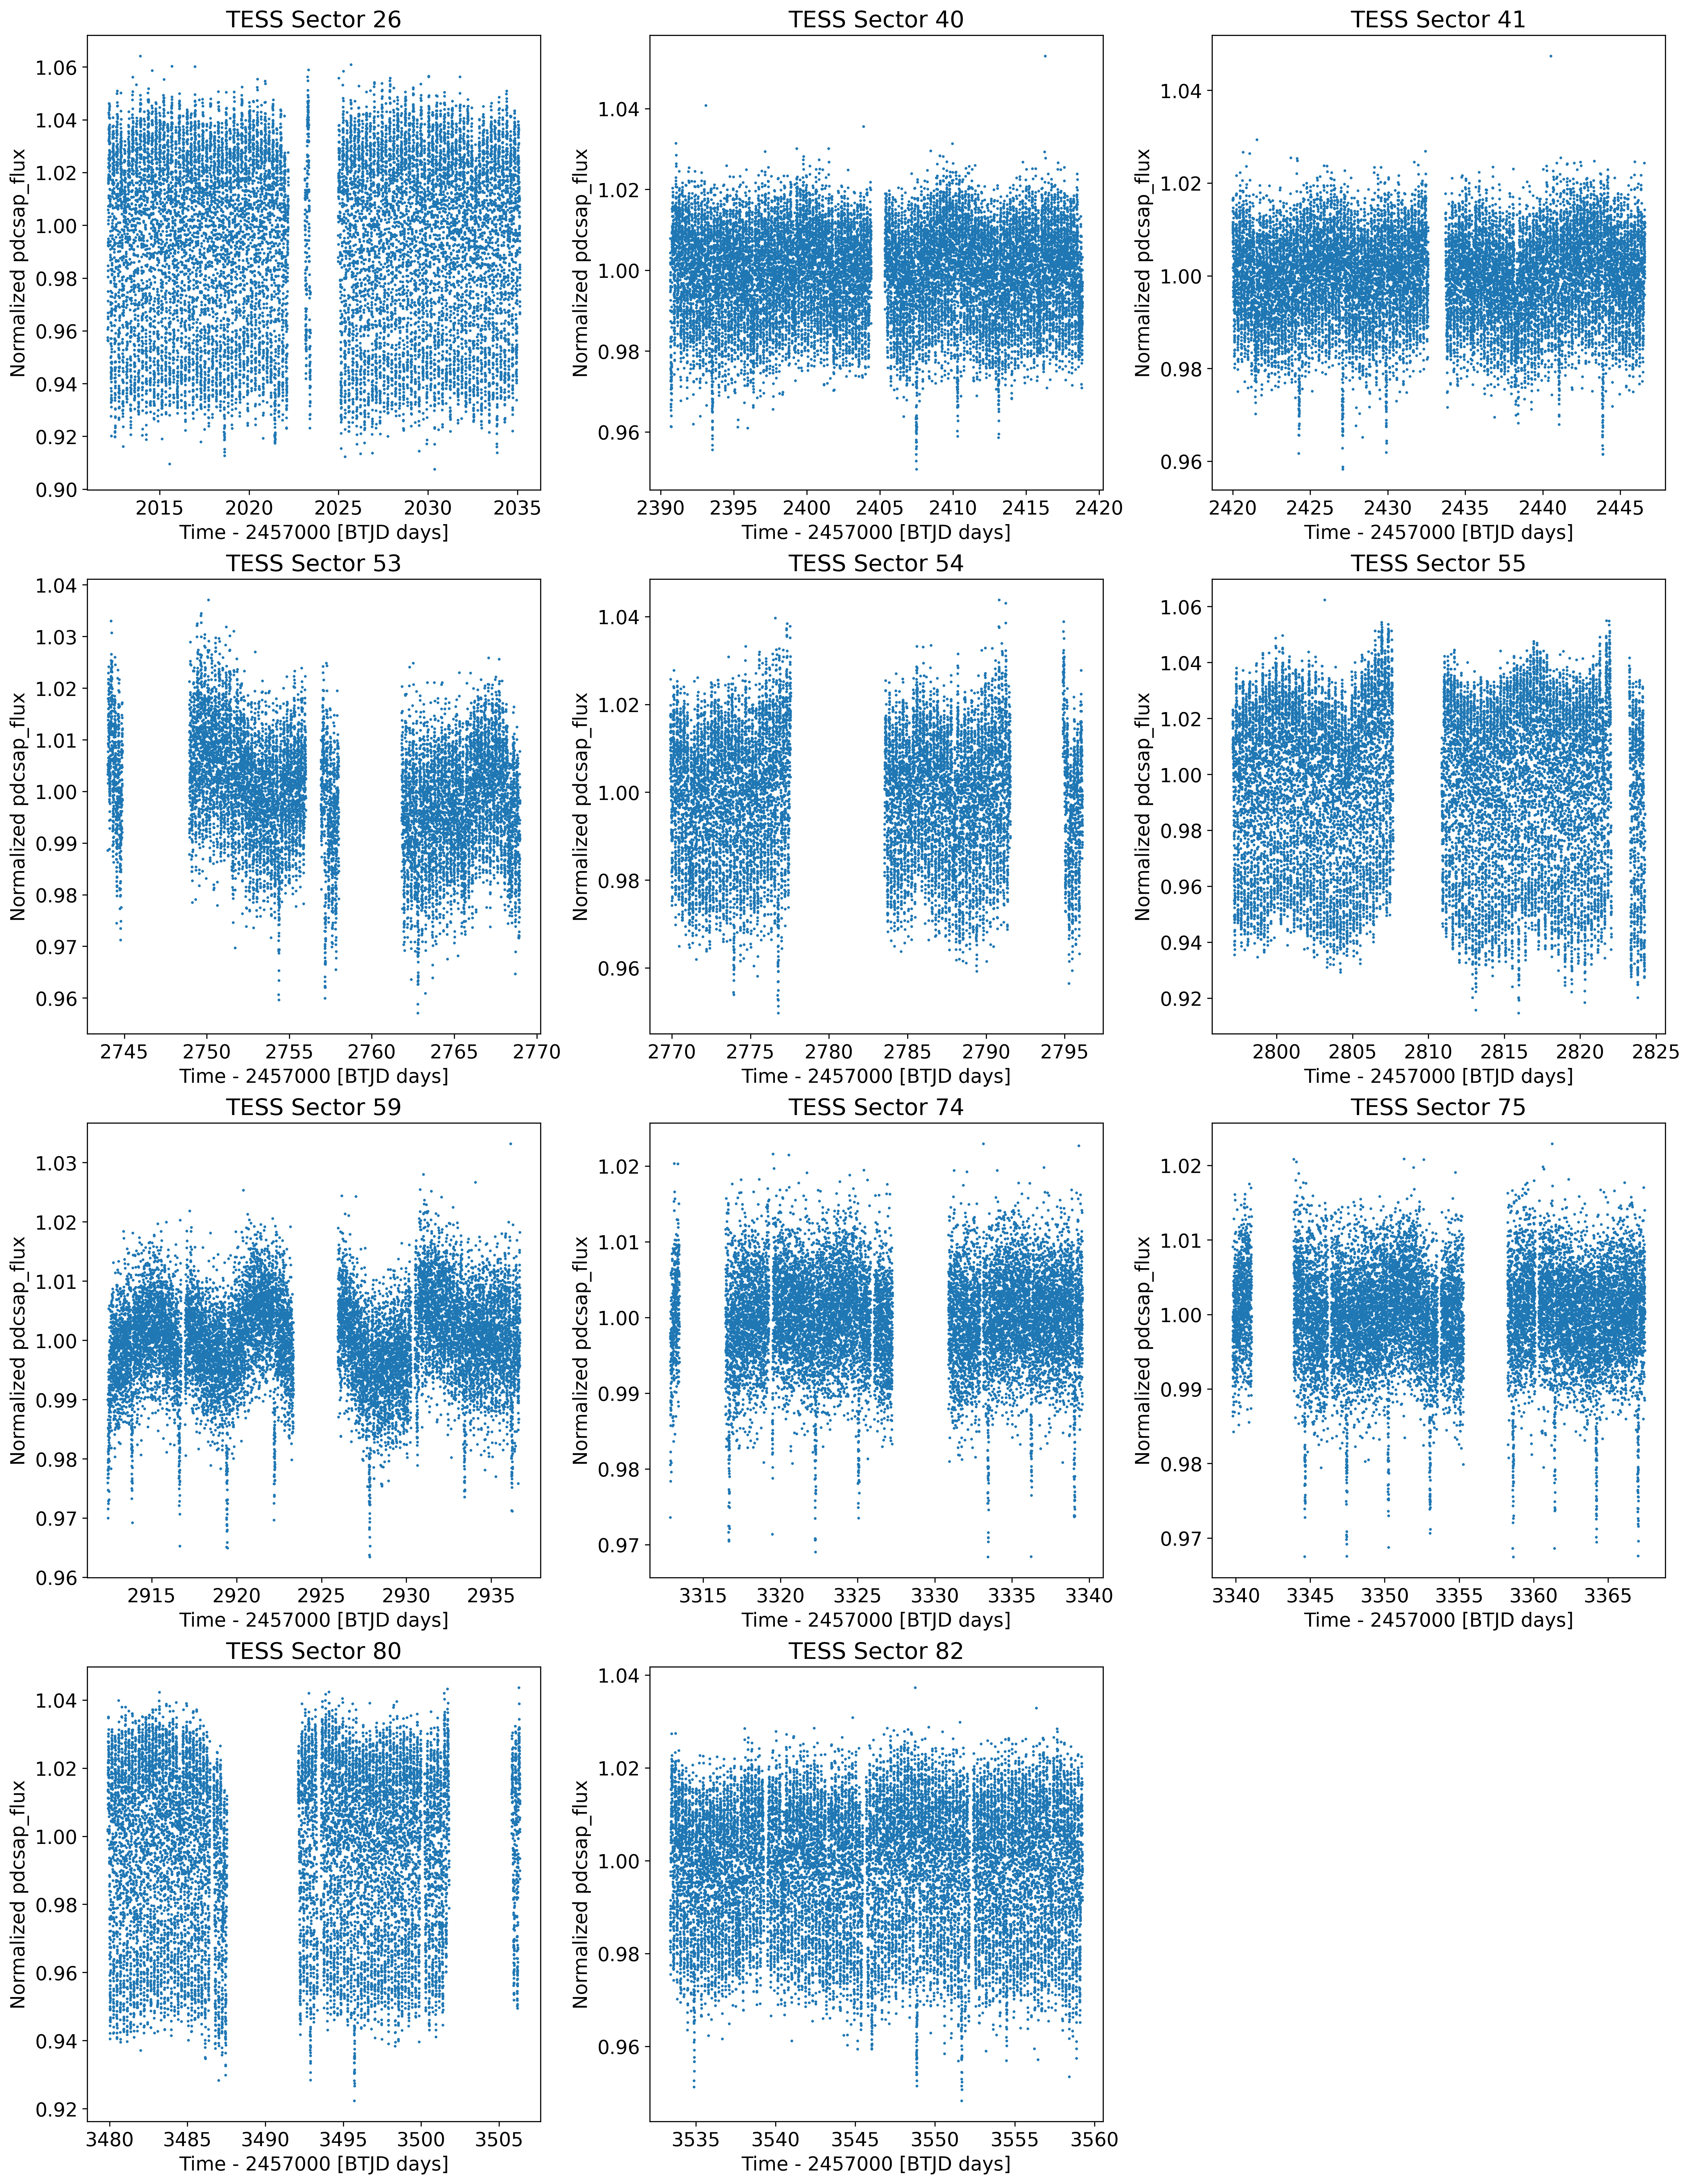
\includegraphics[width=\linewidth]{code/figures/allSectors_sigma5_PDCSAPflux_lc.png}
    \caption{PDCSAP flux for each sector of Tess data}
    \label{fig:enter-label}
\end{figure}

TESS Sectors 74 and 75 did not show significant contamination and were able to be fit using the analysis as described in Adams et. al. \citep{doomed_worlds1}. We also exclude Sector 59 from this analysis and use the mid-times as reported in Wang et. al. 

\begin{figure}
    \centering
    \includegraphics[width=\linewidth]{figures/wellbehaved_sectors_LS_periodogram.png}
    \caption{Lomb-Scargle Periodogram of the TESS sectors used in this study. Each sector returns a period at maximum power approximately one-half of the expected period of that of the EB.}
    \label{fig:LS}
\end{figure}

For these contaminated sectors, ...

\subsection{Boise State University} \label{sec:BSU}
\subsubsection{SuPerPiG Observing Grid}
\COM{6? midtimes}

\subsubsection{Campus Observatory}
\COM{? midtimes}

\subsubsection{Bruneau Dunes State Park}
\COM{1 midtime}

\subsection{Arizona State University Program} \label{sec:ASU}
\COM{13 midtimes}
\COM{Heather/Fred please describe your observation/analysis methods here}

\subsection{Unistellar Citizen Science Program} \label{sec:CitSci}
\COM{? midtimes}
\COM{Lauren please describe your observation/analysis methods here}

\section{Analysis} \label{sec:analysis}

\section{Discussion \& Conclusions} \label{sec:conc}

% \section{Supplemental}

\subsection{Individual Detrended Transit Light Curves by Sector}

\subsubsection{Sector 26 - Currently not in Delta BIC calculations}
\begin{figure}[htbp]
    \centering
    \includegraphics[width=0.5\linewidth]{figures/S26/fitted_transitHATP37b_20200615-08.png}
    \caption{Detrended and Fit Light Curve for Epoch 1205}
    \label{fig:S26-E1205}
\end{figure}

\begin{figure}[htbp]
    \centering
    \includegraphics[width=0.5\linewidth]{figures/S26/fitted_transitHATP37b_20200618-03.png}
    \caption{Detrended and Fit Light Curve for Epoch 1206}
    \label{fig:S26-E1206}
\end{figure}

\begin{figure}[htbp]
    \centering
    \includegraphics[width=0.5\linewidth]{figures/S26/fitted_transitHATP37b_20200626-13.png}
    \caption{Detrended and Fit Light Curve for Epoch 1209}
    \label{fig:S26-E1209}
\end{figure}

% \begin{figure}
%     \centering
%     \includegraphics[width=0.5\linewidth]{figures/S26/fitted_transitHATP37b_20200629-08.png}
%     \caption{Detrended and Fit Light Curve for Epoch 1210}
%     \label{fig:S26-E1210}
% \end{figure}


\begin{acknowledgments}
RMH was supported by the NASA Citizen Science Seed Funding Program, award number XX and the NASA Science Activation Program, award number 80NSSC22M0008. BJ, AK, DC, ERA, AS, and JPM were supported by a grant from the NASA Exoplanets Research Program, award number 80NSSC22K0317. MB was supported by the Idaho Space Grant Consortium. \COM{Add your acknowledgements please :)}
\end{acknowledgments}

\software{lightkurve \citep{lightkurve:2018}, astropy \citep{astropy:2013, astropy:2018, astropy:2022},
astroquery, tesscut, matplotlib \citep{Hunter:2007}, numpy \citep{harris2020array}, scipy \citep{2020SciPy-NMeth}}

\appendix

\section{Appendix}

\bibliography{HATP37b_TransitTiming}{}
\bibliographystyle{aasjournalv7}


\end{document}

% End of file `sample7.tex'.
